\chap{Counters}
\section{Part V}
\begin{itemize}
    \item []\textbf{REQUIREMENT}
        \begin{enumerate}
            \item Augment your circuit from Part IV so that it can rotate the word over all of the 7-segment displays on your DE-series board. 
            \item The shifting pattern for the DE10-Lite is shown in Table below. Your can base on this table to create your own table for DE2i-150.
                \begin{figure}[h]
                    \centering
                    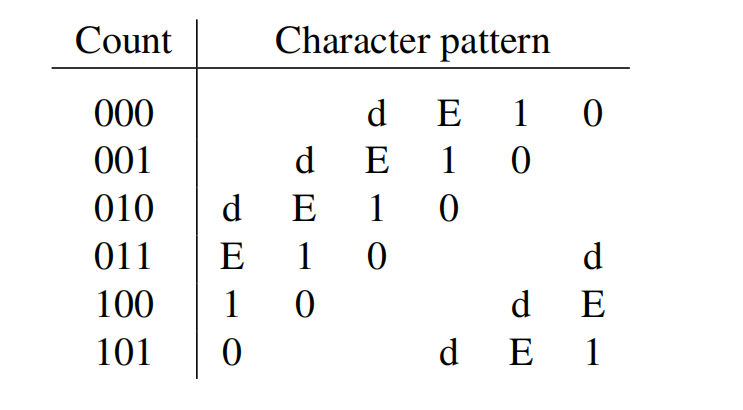
\includegraphics[width=10cm]{source/picture/lab4/Lab4_table1.png}
                    \caption{Rotating the word on six display}
                \end{figure}
        \end{enumerate}
    \item []\textbf{SOLUTION}
        \begin{itemize}
            \item []To use the clock of the board which has the frequency equal to 50MHz, we have to create the counter with in the input is the board’s clock and the output which just equal to 1 when                    
                \begin{lstlisting}[language = verilog]
always @(posedge CLK) begin
    if (Q == 50000000) flag<=1;
    else flag <= 50000000;
    
    if (!CLR | Q>50000000)  Q<= 0;
    else if (EN) Q <= Q + 1;
end

always @(posedge flag) begin
    if (!CLR | C>7)  C<= 0;
    else if (EN) C <= C + 1;
end
                    \end{lstlisting}
            \item []Each time the output of the counter equal to 1, we update the value of 8 7-segment leds by follow module.
                \begin{lstlisting}[language = verilog]
module update_display(out, val);
	input [2:0]val;
	output[55:0]out;
	
	wire [55:0]temp = 56'b111111111111111111111111111110100001000011001001001111011;
	wire [55:0]templong = temp<<(7*val);
	wire [55:0]tempshort = temp>>(56-7*val);
	
	assign out = templong | tempshort;

endmodule
                    \end{lstlisting}
            \item[]Ansd this is the entire design
                \begin{lstlisting}[language = verilog]
always @(posedge CLK) begin
    if (Q == 50000000) flag<=1;
    else flag <= 50000000;
    
    if (!CLR | Q>50000000)  Q<= 0;
    else if (EN) Q <= Q + 1;
end

always @(posedge flag) begin
    if (!CLR | C>7)  C<= 0;
    else if (EN) C <= C + 1;
end
always @(HEX_BUS) HEX = HEX_BUS;


update_display inst1(.out(HEX_BUS), .val(C[2:0]));
assign {HEX7,HEX6,HEX5,HEX4,HEX3,HEX2,HEX1,HEX0} = HEX;
                \end{lstlisting}
            \end{itemize}
    \item[]\textbf{VERIFICATION}
        \begin{figure}[h]
            \centering
            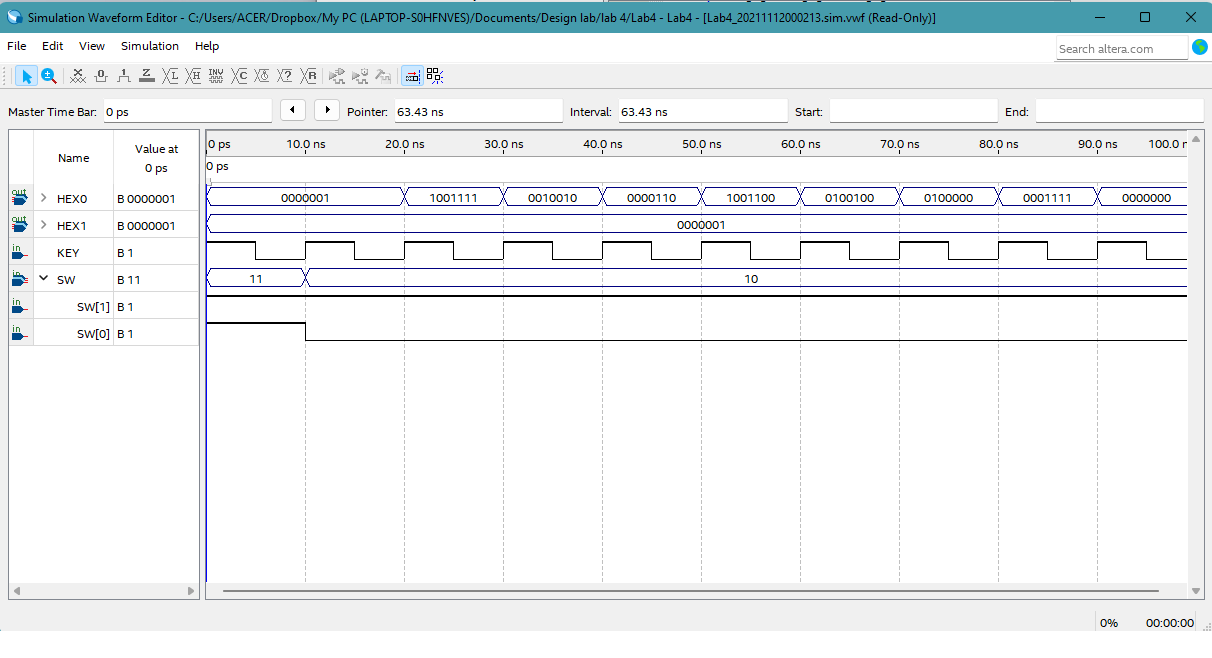
\includegraphics[scale = 0.5]{source/picture/lab4/part1.png}
            \caption{Simulation result}
        \end{figure}
\end{itemize}
\clearpage